\documentclass[a4paper]{report}

\usepackage{amsmath}
\usepackage{amssymb}
\usepackage{graphicx}
\usepackage{hyperref}
\usepackage[top=1in, bottom=1.25in, left=1.25in, right=1.25in]{geometry}

\begin{document}
  \begin{titlepage}
  \title{Quantum Dots Thermometry}
    \author{Biplab Mahato}
    \date{}
    \maketitle
  \end{titlepage}
  
  \section*{Introduction}
    \hspace{10pt} In last two decades study of quantum dots gained an enormous attention in condensed matter physics. Promising use of it in nanoelectronics as well as computation attracted attention of many great minds  across the world. Its a high end techno-intensive experimental field of science. Yet purely theoretical understanding of it is also interesting. My summer project is on the theoretical aspects of quantum dots, especially on \emph{Coulomb-blockade oscillation}. The report is intended to give a short introduction to the realm of Coulomb-blockade following the footsteps of \emph{Beenakker}'s paper\`{ref2}. Report ends with the analysis of the data taken from an experiment.
    
  \section*{2DEG:}
    \hspace{10pt} Study of quantum dots may be started with the study of \emph{two dimensional electron gas (2DEG)}. Electrons in two dimensional electron gas is constrained to move in a plane due to strong electrostatic confinement. This can be achieved in Si-inversion layer or in GaAs-AlGaAs heterostructure. In both the cases a triangular potential well is created in the junction of heterostructure where electrons are trapped. This takes away one degree of freedom of  electrons in the junction. Inside the well electrons behave as if free particle in 2D analogous to ideal gas molecule in a container(3D). Hence the name. Electron density in 2DEG $n_{s}$ can be varied continuously by applying voltage using a gate placed parellel to the plane of confinement as follows
    \begin{equation}\label{eqn1}
      \delta n_{s} =  \dfrac{\epsilon}{ed} \delta \phi_{gate}
    \end{equation} 
    \hspace{10pt} 2DEG can be given any desired shape with the help of \emph{lithographic technique}(e.g.Molecular beam epitaxy). Either by permanently removing electrons or by depleting electron density using electrostatic potential using patterened gate.
    
  \section*{Quantum Dots}
    \hspace{10pt} Quantum dots are made by restricting\footnote{applying voltages through patterened gates according to eqn\ref{eqn1}} 2DEG in a very small \footnote{$\approx 100$ nm dimension} region. This region is weakly coupled\footnote{electron cannot flow freely through the junction it has to tunnel across. Quantitatively finite width of the dot $h\Gamma$ should be much less than $k_{b}T$ i.e. $h\Gamma \equiv h(\Gamma^l + \Gamma^r) \ll k_{b}T$} with two reservoirs known as \emph{source} and \emph{drain}. Reservoirs are large pool of free electron compared to QD which contains around a few hundreds electrons. A gate is also connected to the system which is used to change the potential of the dot (see fig1).
    \begin{figure}[h]
      \centering
      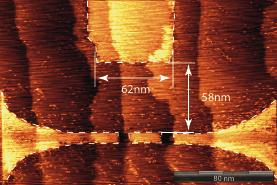
\includegraphics[scale=0.7]{image/df}
      \caption`{Quantum dot carved on a silicon surface with phosphorus as dopant.  Block in the center is the dot which is connected to two reservoirs on both side. A gate is connected shown in the top center position of the figure}
    \end{figure}
    Quantum dots can show numerous interesting phenomenon among them conduction of electrons through it of special interest to this report.

  \section*{Coulomb Blockade Theory}
    \hspace{10pt} Conductance through QD at low temperature is described by Coulomb Blockade theory. This theory can be illustrated by taking a simplified model popularly known as \emph{Constant Interaction Model}. This model assumes That two reservoirs are coupled to the dot with constant capacitance $C_{dot}$ and the gate is coupled with capacitance $C_{gate}$.  Energy levels in the dot is discrete since the electrons are forced to be inside the dot. Let $E_{p}$ denote the energy of the $p^{th}$ energy state. Note that level spacing $\Delta E$ may not be constant; it can even vanish in case of degeneracy. \\
    In the reservoirs electrons are assumed to be \emph{freely} moving  in two dimension(taken as x-y plane). So it is coustomary to assume that electrons obey fermi distribution. Hence at very low temperature most of the electron have energy equal to fermi energy $E_{F}$. 

    \subsection*{Coulomb Blockade oscillation}
      \hspace{10pt} We are interested in the process of conductance through the dot. To do so let's first consider the equlibrium condition. \\
      The probability $P(N)$ to find N electrons in the dot in equilibrium with the reservoirs is given by the distribution 
      \begin{equation} \label{eqn2} 
        P(N) = p\times exp\left( -\frac{1}{k_{b}T} [F(N)-NE_{F}]\right)
      \end{equation}
      where p is normalising constant $F(N)$ is the free energy of the dot and T is temperature. To have conduction then we need nonvanishing $P(N)$ and $P(N+1)$. Because then only no of electrons in the dot can change from N to N+1 giving positive conductance. For that we should have 
      \begin{equation} \label{eqn3}
        F(N)-NE_{F}=F(N+1)-(N+1)E_{F} \\
        \Rightarrow F(N+1)-F(N)=E_{F}
      \end{equation}
      Free energy of the dot comprises  the internal energy of the electron inside the dot in addition with the energy corresponds to external applied voltage $\phi_{ext}$.
      \begin{equation}\label{eqn4} 
        F(N) = \dfrac{(Ne)^2}{2C} + \Sigma_{i=1} ^N E_{p} -Ne\phi_{ext}
      \end{equation}
      where first two terms represent the interaction energy among the electrons inside the dot and the last term is energy due to gate voltage. Here C is the total capacitance of the dot $C = C_{dot}+C_{gate}$. Also it should be noted that $\phi_{ext}$ is not equal to the applied gate voltage but proportional to it $\phi_{ext} = constant + \alpha \phi_{gate}$. where $\alpha = C_{gate}/C$ is known as lever arm of the dot. Now substituting \ref{eqn4} in \ref{eqn3} 
      \begin{equation} \label{eqn5}
        E_{N+1} + \dfrac{e^2}{C}\left(N+\frac{1}{2}\right) = E_{F} + e\phi_{ext}
      \end{equation}
      left hand side is termed as renormalised energy level which gives renormalised energy level separation $\Delta E^* = \Delta E + e^2/C$. This equation suggests that conduction peak is observed with the separation $\delta \phi_{ext} = \Delta E^*/e$. That is conduction peaks are separated by $\Delta E^*/e$. Three cases arises in this point
      \begin{itemize}
        \item \textbf{$\Delta E \gg e^2/C$}  	In this case conduction only happen when energy level of the dot align with  $E_{F}$. This kind of conduction is called \emph{ resonant tunneling}. Spacing in conduction peak is just the level spacing in this perticular case.
        \item \textbf{$\Delta E \ll e^2/C$} A periodic spacing in conduction peak is seen here with spacing corresponds to charging energy $e^2/C$. This case termed as classical \emph{ Coulomb Blockade oscillation}.
        \item \textbf{$\Delta E \approx e^2/C$} Peaks are not periodic but spaced by $\Delta E^*/e$. 
      \end{itemize}
      So now we have renormalised energy levels separeted by $\Delta E^*$ . Whenever right hand side of \ref{eqn5} becomes equal to the renormalised energy level conduction happens i.e. we get conduction peak.
      Right hand side of \ref{eqn5} has two component. $E_{F}$ is dependent on voltage of the reservoirs while $\phi_{ext}$ can be varied using gate voltage.  
      Keeping fixed $E_{F}$ if we vary gate voltage continuously then several separeted conduction peaks are obtained.\\
      Several modification can be made to this simple model. Random fluctuation due to non-zero temperature of electrons changes the exact shape of the peaks at some specific gate voltages. Sudden jump in conductance is removed by smooth transition from zero conductance to heighest conductance and then back to zero. \\
      Conduction may not happen only through resonance tunneling but may happen due to \emph{co-tunneling}. When the system is not in its any of the resonant position then also electron can tunnel into the dot with higher energy. But that electron cannot stay there for long it will tunnel back to the reservoirs. The energy fluctuation in the process and the time scale are given by Heisenberg's uncertainty principle $\Delta E \Delta t \geq \frac{h}{4\pi}$. This co-tunneling is held responsible for non-zero conductance even in the halfway between two peaks(see fig2).
    \subsection*{Amplitude and Lineshape}
      \hspace{10pt} As described in previous section high temperature may ruin the oscillation pattern. So we need much low temp i.e. $k_{b} T < max(\Delta E,e^2/C)$. Two extreme cases arises.\footnote{These two cases are called respectively as quantum regime and classical regime. This is because in second case $\Delta E $ is much less than charging energy, giving essentially continuous energy levels like any typical classical system. Whereas  in the first case it is other way round discretisation of energy create quantum effects hence the name.}
      \begin{itemize}
        \item $k_{b} T \ll \Delta E$ In this case only a single energy level of the dot align with the $E_{F}$ giving conductance. As derived in \ref{ref2} Conductance in this case is given by
        \begin{equation}
          G = \dfrac{G_{max} }{\cosh^2 \left(\frac{\Delta_{min}}{2k_{b}T} \right)}
        \end{equation}
        \begin{equation}
          G_{max} = \dfrac{e^2}{4k_{b} T} \dfrac{\Gamma^l \Gamma^r}{\Gamma^l + \Gamma^r}
        \end{equation} 
        In these equations $\Delta_{min}$ is the minimum value of the function $\Delta(N) = F(N) -F(N-1) -E_{N} -\mu -E_{F} $ where $\mu$ is the chemical potential of the dot. And $\Gamma 's$ are tunneling co-efficient of the junctions of the dot with the left and right reservoirs. 

        \item $\Delta E \ll k_{b} T \ll e^2/C$ In this case as the energy level separations of the dot are small a continuum of levels align to give contribution in conductance. As derived in ref ?? Conductance in this case is given by

        \begin{equation}
          G = \dfrac{G_{max}}{\cosh^2 \left(\frac{\Delta_{min}}{2.5k_{b}T}\right)} 
        \end{equation}
        where $\Delta_{min}$ and $G_{max}$ are same as earlier.
      \end{itemize}

  \section*{Data Analysis}
    \hspace{10pt} Continuing from previous section lineshape of Coulomb blockade oscillation peak has the form of the function $\cosh^{-2} (x)$. So any peak of oscillation can be fitted with function of the form $a+c\left(\cosh^{-2}(b(V_{gate}-V_{0})/2k_{b}T)\right)$. Here $a,b,c,V_{0}$ and T are adaptable parameters. First term  'a' gives the ofset whereas 'b' capture the value of $G_{max}$. Coulomb blockade oscillation and fit using the equation mentioned above is shown\ref{fig2}.
    \begin{figure}[h]
      \centering
      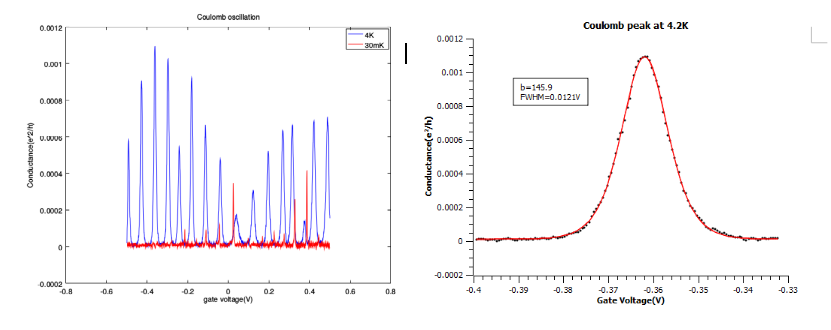
\includegraphics[scale=0.5]{image/cbo1}\label{fig2}
      \caption{Left figure shows Coulomb blockade oscillation at two different temperatures while the right figure shows fitting of a curve of the form $a+c\left(\cosh^{-2}(b(V_{gate}-V_{0})/2k_{b}T)\right)$.}
    \end{figure}
  
    After fitting the curve into the oscillation at various temperature different values of $c/T$ is obtained. Now if we assume at relatively higher temperature temperature of the electron in the dot coinside with the refrigerator temperature then at lower temperature different values of temperature can be obtained which is plotted along with refrigerator temperature\ref{fig3}.
    \begin{figure}[h] \label{fig3}
      \centering
      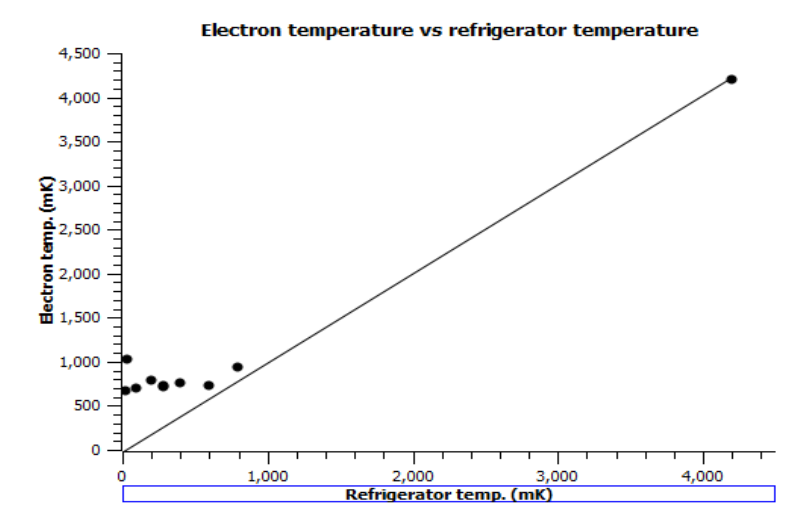
\includegraphics[scale=0.27]{image/rft}
      \caption{Plot of electron temperature vs refrigerator temperature. At low temperature electron temperature become saturated.}
    \end{figure}

    Clearly a saturation of the temperature at lower temperature which is not in accordance to the theory we discussed yet. Main reason for this saturation is the freezing of phonon bath. At extremely low value of temperature vibration of the phonons are very much lowered which prevent heat flow through conduction. So any heat produced inside the dot barely gets the chance to be released through the cooling system of the dilution refrigerator. This causes the temperature of the dot to saturate. \\
    A few assumptions is employed inherently while fitting. We have assumed linear relationship of $\Delta_{min} $ with gate voltage $V_{G}$ which may not be true. Though it gives a farely good insight to the system under observation. Recently many numerical simulated model which takes  every free electrons in the dots into account are comming up\ref{x1}. Such quantum mechanical model will reveal many interesting phenomenon as well as be able to explain existing phenomenona. 

  \section*{What did I learn from it?}
    \hspace{10pt} Personal yield from this mostly theoretical project is very high. Exposure
    to cutting edge research areas is the first to be mentioned. I learned some
    of the theoretical advances in this field like conservation of charge (charging
    energy and Coulomb Blockade oscillation) and conservation of conductance
    (Coulomb staircase). Also learned to appreciate the application of models (like
    constant interaction model) to describe and simulate the system and also to
    critically analyse the hypothesis of the model in terms of the experimental data.
    Project gave some experience in handling data and interpreting them. Inaddition to that I got a little exposure to some of the experimental techniques
    used in this field. Excitement at every moment and the joy of exploration are
    just extras in the project.

  \section*{Acknowledgement}
    \hspace{10pt} I am thankful to Prof. Arindam Ghosh for letting me to work under him and guiding me. My gratitude to Dr. Saquib Shamim for helping and guiding me out throughout the duration of the project and beyond. I also like to thank Soham Ray for doing the project with me.

  \section*{References}
    \begin{enumerate}\label{ref}
      \item   \href{http://physics.aps.org/articles/v3/47}{Viewpoint: \emph{A not-so easy state}}\label{x1}
      \item C.W.J.Beenakker, Phys. Rev. B 44 1646 (1991) \label{ref2}
      \item H. Houten, Beenakker, A. A. M. Staring \textit{Coulomb-Blockade Oscillations in Semiconductor Nanostructures}  arXiv:cond-mat/0508454 v1 \label{ref3}
      \item Gregor Fessler \textit{Electron Temperature in GaAs Quantum Dots} \label{ref4}
    \end{enumerate}
\end{document}